%!TEX TS-program = xelatex

%%%%%%%%%%%%%%%%%%%%%%%%%%%%%%%%%%%%%%%%%%%%%%%%
% CV template
% Originally created by Adrien Friggeri
% Improved by Carmine Benedetto
%%%%%%%%%%%%%%%%%%%%%%%%%%%%%%%%%%%%%%%%%%%%%%%%

\documentclass[]{cv-class}
\usepackage{afterpage}
\usepackage{hyperref}
\usepackage{color}
\usepackage{xcolor}
\hypersetup{
    colorlinks=true,
    linkcolor=blue
}
\RequirePackage{xcolor}
\definecolor{pblue}{HTML}{0395DE}

\begin{document}
\vspace{0.2cm}
\header{Boris }{TRAN}
      {Devops, Project Manager, Architect}

% Fake text to add separator
\vspace{1.15cm}
\fcolorbox{white}{gray}{\parbox{\dimexpr\textwidth-2\fboxsep-2\fboxrule}{%
.....
}}

% In the aside, each new line forces a line break
\begin{aside}
%  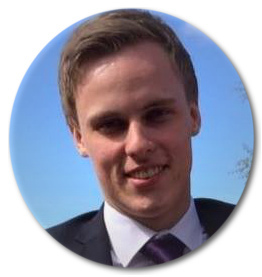
\includegraphics[scale=0.40]{img/meg2.jpg}
  \vspace{0.4cm}
    ~		
  \vspace{0.65cm}
  \section{Mail}
    \underline{\href{mailto:amallyn@pm.me}{amallyn@pm.me}}
    ~
  \section{Phone}
    +33 6 40 43 34 79
    ~
  \section{Address}
    43 Boulevard de Longchamp\\
    Nantes\\
    France (CET)
    ~
  \section{Web}
  	%\underline{\href{http://martinothamar.github.io}{martinothamar.github.io}}
	\vspace{0.10cm}
    \underline{\href{https://github.com/Amallyn}{github.com/Amallyn}}
	\vspace{0.10cm}
    \underline{\href{https://twitter.com/Amallyn1}{twitter.com/Amallyn1}}
	\vspace{0.10cm}
    \underline{\href{https://www.linkedin.com/in/boristran}{www.linkedin.com/in/boristran}}
    ~
  \section{Profile}
    \\
    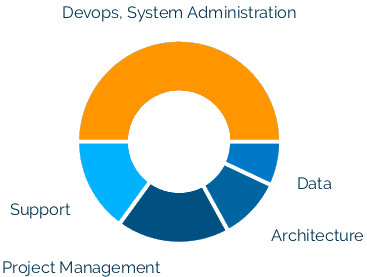
\includegraphics[scale=0.8]{img/skills.png}
    ~
  \section{Languages}
    \\
    \textbf{French}: Native\\
    \textbf{English}: C1\\
    \textbf{Japanese}: A2
    ~
\end{aside}

\vspace{0.4cm}
\section{Experience}
\begin{entrylist}
  \entry
    {2021 - 2022}
    {Project Manager}
    {French Foreign Ministry, France}
    {Our team is in charge of operations and supply chain management, hardware and software 	    tests and support for our Embassies servers.\\
    Project management also encompasses processes optimization between departments. I worked on \textbf{Data visualization tools} for decision taking to \textbf{optimize} our \textbf{operations management}.  A Proof of concept using \textbf{Grafana}, \textbf{Prometheus} and a Python custom exporter led to an in-house software customization.\\
    Maintaining a customized Debian distribution. Package deployment and configuration is handled by \textbf{Ansible}. CI with gitlab has yet to be researched.\\}
  \entry
    {2019 - 2021}
    {System and Network Administrator, Support}
    {French Embassy in Thailand}
    {Handling the \textbf{Covid crisis} demonstrated the challenges of offering \textbf{quick responses} despite the lack of readiness and user training in \textbf{remote solutions}.\\
    In a fast evolving environment, making full use of all the resources at disposal and priority management are essential while safeguarding security standards.\\}
  \entry
    {2015 - 2019}
    {System and Network Administrator, Support}
    {French Mission to the UN, NYC}
    {\textbf{Multilateral Diplomacy} is a very challenging environment.
    System and network administration reaches extremely \textbf{high security standards}.\\
    User support is paramount especially during heads of states events like the United Nations General Assembly, their satisfaction is greatly satisfying.\\
    I continued some prior research and tests on \textbf{containers} (Docker and LXC). \\}
  \entry
    {2011 - 2015}
    {Devops, System Administrator}
    {French Foreign Ministry, France}
    {At the dawn of devops adoption, after \textbf{taking ownership of the servers} infrastructure, \textbf{I researched devops tools} (ansible, salt, puppet, chef).\\ I carried \textbf{tests to deployment and processes migration} on the infrastructure. Since then, its evolution and wide adoption is one of the achievements I am mostly proud of. \\}
  \entry
    {2010 - 2011}
    {System and Network Administrator, Support}
    {French Institute in the UK, London}
    {I researched, designed the architecture and deployed \textbf{high availability virtual servers} (Linux Kvm).\\
    System administration encompassed \textbf{Samba/Ldap}, the French Institute library and cinema softwares, Nas backups. I maintained and prepared the network on a 3-site architecture prior to a future VOIP deployment. \\}
  \entry
    {2006 - 2010}
    {Webmaster}
    {French Embassy to the United Kingdom, London}
    {In the Press Department, I led the France in the United Kingdom webmaster team to merge all websites into a single one. I developed merging tools in \textbf{Python} for database and media.\\
I communicated best practices (XHTML, CSS), maintained high availability of the website and supported users.
I negociated with Hosting providers to improve quality of service and reduce costs. \\}\end{entrylist}
\begin{entrylist}
  \entry
    {2006}
    {Quality Assurance Tester}
    {Square Enix, London}
    {Translation proof reading from English and Japanese to French. Bug reporting \\}  \entry
    {2002 - 2004}
    {Business creation of a specialized computer parts online shop}
    {France}
    {I improved a \textbf{LAMP} template website,  managed hosting.\\
    \textbf{Stock management and logistics} were the most challenging tasks. \\}
\entry
    {2000 - 2001}
    {R\&D Developer}
    {Duran, Paris}
    {As a team member, I worked on Virtual Observer, an online 3D Real Time application for following the Vendée Globe skipper race (\textbf{VC++, OpenGL, SQLServer}). I prototyped a small physics library and developed 3D optimization for \textbf{Virtual Skipper 2}, a skipper racing game. \\}
  \entry
    {1999 - 2000}
    {Game Developer}
    {Eden-Studios, a development studio, France}
    {I developed a 3D audio library for \textbf{V-Rally 2 PC}, a rally driving game. (\textbf{VC}) \\}
\end{entrylist}
    
\section{Education}
\begin{entrylist}
  \entry
    {2005 - 2006}
    {Cambridge Certificate in Advanced English}
    {London}
    {Cambridge First Certificate in English (FCE) and Certificate in Advanced English (CAE).\\}
  \entry
    {1998 - 1999}
    {1-year postgraduate diploma}
    {UNIGE, EPFL, Switzerland, Lyon I University, France}
    {Computer Graphics and Networks\\
    European diploma in Computer Visualization and communication, EPFL Lausanne, UNIGE Geneva, Switzerland, Lyon I University, France\\}
  \entry
    {1994 - 1998}
    {M.Sc., B.Sc. and 2-year undergraduate diploma}
    {Lyon I University, France}
    {Mathematics, Science and Computer Science\\}
\end{entrylist}

\begin{aside}
  \vspace{1cm}
  \section{Skills}
    \\
    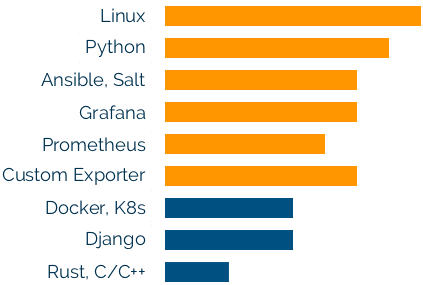
\includegraphics[scale=0.68]{img/skills2.png}    ~
\end{aside}



\section{Projects}
\begin{entrylist}
  \entry
    {2021 - 2022}
    {Kusama Validator Node Administration}
    {Blockchain}
    {I maintain two Kusama Validator Nodes using Ansible.\\
    I also research other nodes stack.\\}
  \entry
    {2021}
    {Tor network crawler and search engine}
    {Tor, Python, Docker}
    {For this spare time project, I developed a Tor network crawler and search engine practicing \textbf{Python} and \textbf{Docker}. \underline{\href{https://github.com/Amallyn/torcrawler}{github.com/Amallyn/torcrawler}}.\\}
  \entry
    {2017 - 2019}
    {POW Mining}
    {Blockchain}
    {Building nodes and miners from code was mandatory for mining. I did light customization of a Linux distribution and miners to optimize performance.}
\end{entrylist}

%\vspace{1.5cm}
%\end{flushright}
%\begin{flushright}
%\emph{\today}
%\end{flushright}

\end{document}
